\header{
    \headtitle{Un petit Ricard} \label{le-petit-ricard}
    %
    
    \insertComment{Chanson de Ricoune (2002).}{}
}

\enluminure{4}{\href{https://www.youtube.com/watch?v=ZiHHcUNc3P8}{Q}}{uand} je suis entré dans le bar
\\Il était midi moins le quart
\\Je me suis assis au comptoir
\\J'ai commandé un petit ricard
\\\\Tous les clients m'ont regardé
\\Ils m'ont pris pour un vrai marseillais
\\Quand j'ai sorti mon billet de 100 francs
\\Ils se sont moqués de mon accent !
\\\\\textbf{Refrain :}
\\Je voudrais un petit ricard dans un verre à ballon
\\Laissez moi le consommer avec modération
\\On va pas se disputer pour payer l'addition
\\Je partirai pas sans boire la tournée du patron
\\Ca fait parti des coutumes et des traditions !
\\Avant de rentrer de la maison
\\Un Ricard sinon rien et je reviendrai demain
\\\\Pendant que le curé fait la messe
\\Pendant qu'il s'occupe de nos gonzesses
\\Nous on fait la prière du matin
\\Donnez nous notre Ricard quotidien
\\\\Il faut surtout pas oublier
\\Les olives et les petits salés
\\Demandez gentiment au patron
\\De vous le servir avec un glaçon
\\\\Quand je suis ressorti du bar
\\Il était midi moins le quart
\\Ma copine était en colère
\\Elle m'a insulté d'un air sévère
\breakpage
\textbf{Refrain final :}
\\Avec ton petit Ricard tu me mets les ballons
\\Tu vas faire tes valises et quitter la maison
\\Ca fait déjà longtemps que je te mets la pression
\\Et ça rentre dans l'oreille et ça ressort à fond
\\N'oublie pas tes chemises et tes pantalons
\\Avant de partir de la maison un Ricard sinon rien
\\Et on se revoit jamais.... et jamais...
\\
\begin{center}
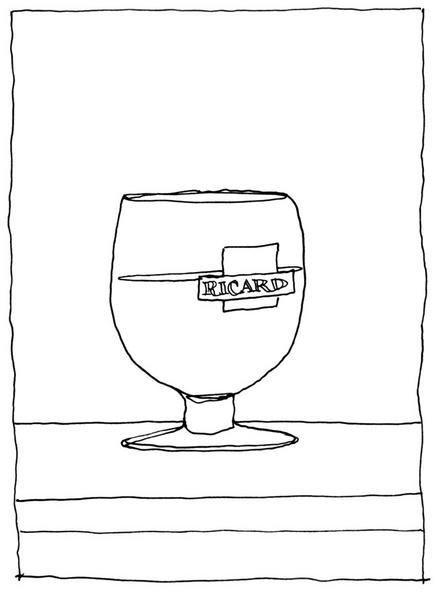
\includegraphics[width=0.8\textwidth]{images/Ricard.jpg}
\end{center}

\breakpage